\section{Introduction}
During recent years, a number of studies have shown how introducing clicker systems, also known as Classroom Response System (CRS), can have a positive effect on learning outcomes and classroom interactivity \cite{yourstone2008classroom, siau2006use, lantz2014effectiveness}.

The idea of CRSs is not a new one, and low tech paper based versions have been used in classrooms before. The system is simple, where students hold up a piece of paper, called a response card, with their answer \cite{ralph1994effects}. During the last decade more modern versions of this system has been introduced, the so called \emph{clickers}. A clicker in it's most basic form, is a device that allows the users to respond to questions, most commonly in a classroom environment. Such a system has been defined by \citeA{lantz2014effectiveness} as 

\begin{quote}
    \emph{"[...] individual response devices held by individual students allowing them to quickly and anonymously respond to multiple choice questions presented in class. A receiver attached to a classroom computer collects and summarizes the responses instantly and projects them graphically onto the screen for students and the educator to see"} \cite[p.~280]{lantz2014effectiveness}
\end{quote}

As described above, the clicker itself is used for gathering collective answers from the students via a physical clicker device. Many different versions of such systems exists\footnote{\url{https://www1.iclicker.com/}, \url{http://www.renaissance.com/products/2know}}. One example of such a system can be seen in figure \ref{fig:iclicker}.

\begin{figure}[H]
\capstart
	\centering
		\frame{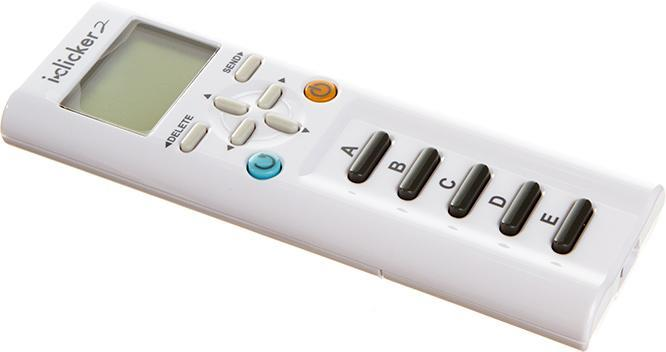
\includegraphics[width=\textwidth]{iclicker.jpg}}
        %\missingfigure{iClicker - An example of an iClicker}
	\caption[iClicker2]{One example of a clicker device called the iClicker2.}\label{fig:iclicker}
\end{figure}

The device depicted in figure \ref{fig:iclicker} is a hardware based CRS, that connects to a receiver in the classroom, that is connected to the teachers computer. The computer can then display the data with a piece of software designed for the system.

A typical hardware based CRS system like the one mentioned above introduces a variety of pros and cons. This includes the investment of buying the system, the receiver and possible licenses for using it could become a large expense. Also there are potential risks, that setting up the system could become a hassle, if the software for example is not maintained for more than one platform or the hardware is difficult to setup. With the emerging of smartphones and fast, reliable internet connections, it could seem like a natural progression to utilize the devices that the users already own, cutting away the expense of buying clicker devices. The users would then use their smartphones or laptops to respond, instead of using a clicker. The concept has been dubbed \emph{Bring Your Own Device} or \emph{BYOD} \cite<Johnson et al., 2013 in>[p.~329]{stowell2015use}. Such systems exists in a variety of different forms, implemented with mixed results. Making the move from the physical to a digital based platform, introduces a whole new range of possibilities and challenges.

There are a variety of examples of online CRS systems. Some are made mainly for children or ground-schoolers\footnote{\url{https://kahoot.it}}, and others are feature rich, made for conferences and classrooms\footnote{\url{http://socrative.com}} \footnote{\url{https://www.polleverywhere.com}} \footnote{\url{https://www.iclicker.com/}}. The most appealing, and seemingly well implemented system is Mentimeter\footnote{\url{https://www.mentimeter.com}}.

Much of the available existing literature about CRS is focused on physical clicker devices and the learning outcomes/improvements of using them. It's less common to find research where the main focus is web based systems, even though smartphones has become widespread and more popular among students \cite[p.~329]{stowell2015use}.

Our own experience shows that it can be problematic when the teacher wants to ask questions which include code. This is hard to do on hardware based devices, and different workarounds where questions are asked on slideshows and answered on clickers are common.


We wish to gain knowledge on how the market is structured today. By using Porters Five Forces \cite{porter2008five}, we will identify possible culprits that we should be aware about when creating such a system, for it to be competitive.

We will then describe the system that we have developed in two parts. First a general introduction to the system. Secondly a technical description of the specific implementation.
We will then perform a test in two different courses: \emph{Frameworks and Architectures for the Web} and \emph{Advanced Programming}. We will discuss our results from the test and show how each CRS performs compared to each other in the two different courses.


\todo{Herfra og ned forsvinder den røde tråd lidt i introduktionen. Tilføj hvad vi gerne vil med det her projekt plus en "walkthrough" af opgavens opbygning}


It would seem that the obvious approach would be to leverage the technology that students already own and use. At the IT University of Copenhagen (ITU), laptops are mandatory and free internet access is provided by the university. 

Each system has a different focus, and how deeply integrated they are varies. Some systems simply wants to ask questions, others wants to grade assignments or provide feedback as well. Though few of them seem to have focus on IT learning specifically, and the ones implementing features that do, lack in other ways.


\subsection{Research question}
We wish to investigate whether a Classroom Response System that is enhanced for IT educational purposes, is able to enhance classroom interactivity and thereby increase the learning outcome. 
We wish to evaluate the system by gathering empirical data by conducting a pre and post survey on students using our system.

